


\documentclass[a4paper, 12pt]{article} 
\usepackage{amsmath, amssymb, color, graphicx, enumitem}
\usepackage{fullpage} %smaller margins
\usepackage{hyperref} % hyperlinks

%font
%\usepackage[sc]{mathpazo}
%\linespread{1.05}         % Palladio needs more leading (space between lines)
%\usepackage[T1]{fontenc}

%font, libertine
\usepackage{libertine}

%word spacing
\usepackage{microtype}

%all equations get full space
\everymath{\displaystyle}

%useful shortcuts
\def\R{\ensuremath{\mathbb{R}}} %\ensuremath adds math mode, if forgotten
\def\Q{\ensuremath{\mathbb{Q}}}
\def\N{\ensuremath{\mathbb{N}}}
\def\Z{\ensuremath{\mathbb{Z}}}
\def\C{\ensuremath{\mathbb{C}}}

%shorcuts with arguments
\newcommand{\abs}[1]{\left\vert#1\right\vert} %nice absolute values
\newcommand{\bt}[1]{\textbf{#1}} %bold
\newcommand{\eq}[1]{\begin{align*}#1\end{align*}} %aligned equations
\newcommand{\cb}[1]{\centerline{\fbox{#1}}} %centered box
\newcommand{\bp}[1]{\fbox{\parbox{0.8\textwidth}{#1}}} %box paragraph
\newcommand{\norm}[1]{\left\lVert#1\right\rVert} %vector norm
\newcommand{\notimplies}{% does not imply
  \mathrel{{\ooalign{\hidewidth$\not\phantom{=}$\hidewidth\cr$\implies$}}}}
\renewcommand{\eq}[1]{\begin{align*}#1\end{align*}} %aligned equations


%colors
\definecolor{javagreen}{rgb}{0.25,0.5,0.35} %dark green color
\newcommand{\green}[1]{\textcolor{javagreen}{#1}} %command for green
\newcommand{\gray}[1]{\textcolor[gray]{0.5}{#1}} %gray text

%environment
\newcommand{\tab}{\phantom{ssss}}


\title{}
\date{}
%==tips====
%part
    %section, sub, sub
%\begin{enumerate}[resume] %continues counting
\begin{document}
\begin{center}
\section*{Quiz 2}
Fundamentals of Calculus I
\end{center}

Name: \underline{\hspace{5cm}} \\

\bt{Explain and justify your thought process.}

Write your answers in the space provided. No calculators allowed.

\begin{enumerate}
    \item Find all solutions to $\frac{1}{e^x} = e^{5(x+2)}$.
    \vspace{6cm}
    \item Solve $\log_5 ((25)^{100}) = (x-1)(x-5) + 195$.
    \vspace{6cm}
    \item What is the minimum value of $x^2 + 8x + 15$ ?
    \vspace{6cm}
    \item Find all solutions to $\log_2 (x^2 - 6x) = 3 + \log_2 (1-x)$.
    \vspace{6cm}
\end{enumerate}


\bt{No justification necessary.}
\begin{enumerate}[resume]
    \item Sketch the graph of $x^{100} + \pi$.
    \vspace{5cm}
    \item Provide one application where logarithms are useful.
    \vspace{5cm}
\end{enumerate}

\bt{True or False. No justification necessary.}
\begin{enumerate}[resume]
    \item \underline{\hspace{1.5cm}} The horizontal asymptote of $\frac{4}{x-5} + 8$ is 5.
    \item \underline{\hspace{1.5cm}} $\log_a (x + y) = \log_a (x) * \log_a (y)$
    \item \underline{\hspace{1.5cm}} The domain of $\log_3 x$  is all real number except 0. \\
\end{enumerate}

\bt{Bonus} (+1 point): How many digits are in $8^{1000}$ ? (hint: $\log 2 = .3010$) 

\newpage

\section*{Solutions}

\bt{Explain and justify your thought process.}

Write your answers in the space provided. No calculators allowed.

\begin{enumerate}
    \item Find all solutions to $\frac{1}{e^x} = e^{5(x+2)}$.

    \green{
    We want to find $x$ values such that 
    \eq{
    e^{-x} = e^{5(x+2)}.
    }
    So, $-x = 5x + 10 \implies -5/3$.
    }
    \item Solve $\log_5 ((25)^{100}) = (x-1)(x-5) + 195$.

    \green{
    Using the definition of $\log$, we have
    \eq{
    5^{(x-1)(x-5)+195} &= 25^{100} \\
    & = 5^{200}.
    }
    Therefore, $(x-1)(x-5) + 195 = 200$, meaning $(x-1)(x-5) = 5$. \\
    Now we solve, 
    \eq{
    x^2 -6x + 5 = 5 \implies x(x-6) = 0 
    }
    So we have $x = 0$ or $x = 6$.
    }
    \item What is the minimum value of $x^2 + 8x + 15$ ?

    \green{
    We can determine the minimum value by relating the function to $x^2$: 
    \eq{
    x^2 + 8x + 15 &= (x+4)^2 -1 
    }
    The function is $x^2$ shifted to the left by 4 and down by -1.  \\
    Therefore, the minimum value of the function is -1.
    }
    \item Find all solutions to $\log_2 (x^2 - 6x) = 3 + \log_2 (1-x)$.

    \green{
    We can rewrite the equation as 
    \eq{
    \log_2(x^2 - 6x) - \log_2(1-x) = 3.
    }
    Next we rewrite the logarithms as 
    \eq{
    \log_2(x^2 -6x) + \log_2(1-x)^{-1} &= 
    \log_2((x^2 - 6x)(1-x)^{-1}) = 3.\\
    }
    By the definition of $\log$ we have
    \eq{
    2^3 = (x^2 - 6x)(1-x)^{-1}
    }
    So, 
    \eq{
    8 - 8x = x^2 -6x \implies x^2 +2x - 8 = 0\\
    \implies (x+1)^2 -9 = 0 \implies x = 2 \text{ or } x = -4
    }
    **NOTE**
    If you're a careful student, you should notice $x=2$ is not in the domain of 
    our original equation, since $\log_2(1-2) = \log_2(-1)$, which is impossible.
    You should reject this solution. The only solution is $x=-4$. 
    Because I'm so very nice, I didn't take any points off this time.
    }
\end{enumerate}


\bt{No justification necessary.}
\begin{enumerate}[resume]
    \item Sketch the graph of $x^{100} + \pi$.

    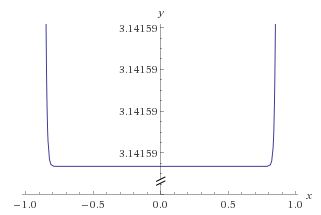
\includegraphics{graphs/x_100_pi.png}

\green{    The shape is parabolic with a y-intercept of $\pi$.}
    \item Provide one application where logarithms are useful.
    \green{
    Answers can range from measuring PH levels to making large numbers (like the hotness of a pepper) human-friendly.
    }
\end{enumerate}

\bt{True or False. No justification necessary.}
\begin{enumerate}[resume]
    \item \underline{\green{False}} The horizontal asymptote of $\frac{4}{x-5} + 8$ is 5.
    \item \underline{\green{False}} $\log_a (x + y) = \log_a (x) * \log_a (y)$
    \item \underline{\green{False}} The domain of $\log_3 x$  is all real number except 0. \\
\end{enumerate}

\bt{Bonus} (+1 point): How many digits are in $8^{1000}$ ? (hint: $\log 2 = .3010$) \\

\green{
We know $\log 8^{1000}$ is the power we need to raise ten by to get $8^{1000}$. \\
This gives us the number of digits in 10s, 100th, 1000th, $\dots$ places. \\
So 
$8$ has $\log 8^{1000}$ + 1 digits (rounded down). \\
To compute $\log 8^{1000}$ we have
\eq{
\log 8^{1000} &= 100 \log 8 \\
&= 100 \log 2^3 = 300 \log 2  \\
& = 300 * .3010 = 903
}
Therefore, $\log 8^{1000}$ has 904 digits.
}

\newpage

\section*{Common Mistakes}

\begin{itemize}
    \item Basic algebra such as the zero product property. For example in question 2$x(x-6) = 0$ implies $x=0$ or $x=6$, both are solutions.
    \item Confusing the minimum of a parabola with the y-intercept. 
    \item Attempting to find the minimum of $x^2 + 8x + 15$ by setting the expression equal to zero (or trying to plug in zero for x).
    \item Claiming the minimum of $x^2 + 8x +15 $ is 15, because it's the constant.
    \item Incorrectly evaluating logarithms: $\log_5 25 = 2$, not 5.
    \item Ignoring logarithms in an equation. In question 4,  $\log_2 (x^2 -6x) = 3 + \log_2(1-x)$ is rewritten without logs as $x^2 - 6x = 1-x$.
    \item Cancelling $\log$: 
    $\frac{\log_2 (x^2 - 6x) }{\log_2 ( 1-x) } \neq \frac{x^2 - 6x }{1-x}$.
\end{itemize}

\end{document}
